% Figure from MATH 556 notes, section 5. Compile with the notes preamble.
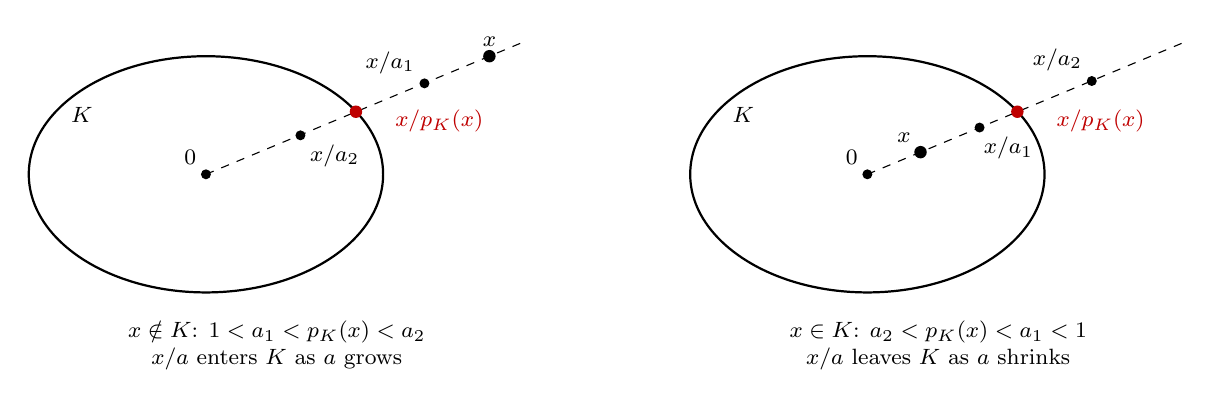
\begin{tikzpicture}[scale=1.5, >=stealth]
    % left: x outside
    \begin{scope}
        \draw[thick] (0,0) ellipse (1.5 and 1.0);
        \node[font=\footnotesize] at (-1.05,0.5) {$K$};
        \draw[dashed] (0,0) -- (2.7,1.125);
        \fill (0,0) circle (1.2pt) node[above left, font=\footnotesize] {$0$};
        \fill (2.4,1.0) circle (1.5pt) node[above, font=\footnotesize] {$x$};
        \fill (1.85,0.77) circle (1.2pt) node[above left, font=\footnotesize] {$x/a_1$};
        \fill[red!75!black] (1.27,0.53) circle (1.5pt);
        \fill (0.8,0.33) circle (1.2pt) node[below right, font=\footnotesize] {$x/a_2$};
        \node[anchor=west, font=\footnotesize, red!75!black] at (1.52,0.45) {$x/p_K(x)$};
        \node[font=\footnotesize, align=center] at (0.6,-1.45) {$x \notin K$: $1 < a_1 < p_K(x) < a_2$ \\ $x/a$ enters $K$ as $a$ grows};
    \end{scope}
    % right: x inside
    \begin{scope}[xshift=5.6cm]
        \draw[thick] (0,0) ellipse (1.5 and 1.0);
        \node[font=\footnotesize] at (-1.05,0.5) {$K$};
        \draw[dashed] (0,0) -- (2.7,1.125);
        \fill (0,0) circle (1.2pt) node[above left, font=\footnotesize] {$0$};
        \fill (0.45,0.1875) circle (1.5pt) node[above left, font=\footnotesize] {$x$};
        \fill (0.95,0.396) circle (1.2pt) node[below right, font=\footnotesize, xshift=-2pt] {$x/a_1$};
        \fill[red!75!black] (1.27,0.53) circle (1.5pt);
        \fill (1.9,0.79) circle (1.2pt) node[above left, font=\footnotesize] {$x/a_2$};
        \node[anchor=west, font=\footnotesize, red!75!black] at (1.52,0.45) {$x/p_K(x)$};
        \node[font=\footnotesize, align=center] at (0.6,-1.45) {$x \in K$: $a_2 < p_K(x) < a_1 < 1$ \\ $x/a$ leaves $K$ as $a$ shrinks};
    \end{scope}
\end{tikzpicture}
